% Presentación final DEFI IV -- compilar con pdfLaTeX en Overleaf.
% Antes de subir a Overleaf ejecute desde la raíz del repositorio:
% python generar_resultados_sustentacion.py \
%   --snapshot-dir informes_pol/snapshot_20260823T014719Z_08 \
%   --rl-dir informes_rl/snapshot_20260823T010000Z_rl_1h_02 \
%   --output-dir presentacion_sustentacion
%
% Luego suba la carpeta completa presentacion_sustentacion/. El archivo
% resultados_ejecucion.tex y las figuras no se editan a mano: son la salida
% de esa ejecución y alimentan todos los resultados empíricos de las diapositivas.

\documentclass[10pt,aspectratio=169]{beamer}

\usetheme{Boadilla}
\usecolortheme{default}
\setbeamertemplate{navigation symbols}{}
\setbeamertemplate{footline}{
  \leavevmode\hbox{%
  \begin{beamercolorbox}[wd=.82\paperwidth,ht=2.6ex,dp=1.2ex,leftskip=1em]{author in head/foot}%
  DEFI IV -- POL/USDC, Polygon
  \end{beamercolorbox}%
  \begin{beamercolorbox}[wd=.18\paperwidth,ht=2.6ex,dp=1.2ex,center]{title in head/foot}%
  \insertframenumber\,/\,\inserttotalframenumber
  \end{beamercolorbox}}%
}

\usepackage[utf8]{inputenc}
\usepackage[T1]{fontenc}
\usepackage[spanish,es-nodecimaldot]{babel}
\usepackage{lmodern}
\usepackage{amsmath,amssymb}
\usepackage{booktabs}
\usepackage{graphicx}
\usepackage{xcolor}
\usepackage{array}

\definecolor{navy}{HTML}{17324D}
\definecolor{blueaccent}{HTML}{2F6B9A}
\definecolor{teal}{HTML}{277A78}
\definecolor{slate}{HTML}{52677D}
\definecolor{lightpanel}{HTML}{EDF3F8}
\setbeamercolor{structure}{fg=blueaccent}
\setbeamercolor{frametitle}{fg=navy,bg=white}
\setbeamercolor{title}{fg=navy}
\setbeamercolor{block title}{fg=white,bg=navy}
\setbeamercolor{block body}{bg=lightpanel,fg=navy}
\setbeamercolor{author in head/foot}{bg=navy,fg=white}
\setbeamercolor{title in head/foot}{bg=blueaccent,fg=white}
\setbeamertemplate{itemize items}[circle]
\renewcommand{\familydefault}{\sfdefault}
% Permite compilar tanto desde la carpeta original como desde el ZIP importado
% a Overleaf, donde los PDF pueden quedar en la raíz del proyecto.
\graphicspath{{./}{figuras/}}

\newcommand{\POL}{\textbf{POL}}
\newcommand{\USDC}{\textbf{USDC}}
\newcommand{\concepto}[1]{\textcolor{blueaccent}{\textbf{#1}}}

% Esta entrada se genera con generar_resultados_sustentacion.py.
% Archivo generado automáticamente. No editar a mano.
% Snapshot wallets: informes_pol/snapshot_20260823T014719Z_08
% Snapshot RL: informes_rl/snapshot_20260823T010000Z_rl_1h_02
\newcommand{\TotalPerfiles}{13\,478}
\newcommand{\TotalGanadores}{631}
\newcommand{\GanadoresUnaHora}{190}
\newcommand{\PerfilesEstrictos}{82}
\newcommand{\WalletsDirigidas}{66}
\newcommand{\EstrictosBuy}{35}
\newcommand{\EstrictosSell}{3}
\newcommand{\EstrictosHold}{44}
\newcommand{\ObservacionesRL}{24}
\newcommand{\TransicionesVerificadas}{48}
\newcommand{\TransicionesValidas}{sí}
\newcommand{\SenalBuy}{3}
\newcommand{\SenalSell}{0}
\newcommand{\SenalHold}{20}
\newcommand{\SenalNeutral}{1}
\newcommand{\PoliticaBuy}{11}
\newcommand{\PoliticaSell}{1}
\newcommand{\PoliticaHold}{12}
\newcommand{\RiquezaInicial}{100.00}
\newcommand{\RiquezaFinal}{113.97}
\newcommand{\RetornoReplay}{+13.97\%}
\newcommand{\ReplayCortes}{24}
\newcommand{\ReplayBuy}{2}
\newcommand{\ReplaySell}{1}
\newcommand{\ReplayHold}{21}
\newcommand{\RiquezaMaxima}{124.86}
\newcommand{\HoraRiquezaMaxima}{22 Ago 08h}
\newcommand{\LaplaceAlpha}{1.00}
\newcommand{\TablaGanadores}{\begin{tabular}{lrrrr}
\toprule
Horizonte & Buy & Sell & Hold & Total \\
\midrule
1m & 38 & 37 & 43 & 118 \\
5m & 75 & 19 & 59 & 153 \\
15m & 88 & 16 & 66 & 170 \\
1h & 98 & 28 & 64 & 190 \\
\bottomrule
\end{tabular}}
\newcommand{\TablaPerfilesDestacados}{\begin{tabular}{llrrrr}
\toprule
Wallet & Acción & $n$ & PnL USDC & Retorno med. & Score \\
\midrule
0x19b5...796c & Buy & 17 & 30.08 & 6.21\% & 0.94 \\
0x4118...53a9 & Sell & 3 & 17.06 & 4.01\% & 0.86 \\
0xd0d0...5bea & Hold & 75 & 86.66 & 4.19\% & 1.00 \\
\bottomrule
\end{tabular}}
\newcommand{\TablaReplayPrimera}{\begin{tabular}{llcrrrrc}
\toprule
Hora UTC & R/W/X & Acción & $X_{t+1}$ & Base & Bono & Final & Riqueza \\
\midrule
22 Ago 02h & FLAT/NEU/0 & Buy  & 1 & +3.6647\% & +0.0000\% & +3.6647\% & 103.66 \\
22 Ago 03h & UP/BUY/1   & Hold & 1 & +6.0858\% & +0.0000\% & +6.0858\% & 109.97 \\
22 Ago 04h & UP/HOLD/1  & Hold & 1 & +5.3438\% & +0.1814\% & +5.5252\% & 116.05 \\
22 Ago 05h & UP/HOLD/1  & Hold & 1 & -2.9488\% & -0.0535\% & -3.0023\% & 112.57 \\
22 Ago 06h & DOWN/HOLD/1& Hold & 1 & +4.6618\% & +0.2233\% & +4.8851\% & 118.07 \\
22 Ago 07h & UP/HOLD/1  & Hold & 1 & +0.6997\% & +0.0202\% & +0.7199\% & 118.91 \\
22 Ago 08h & UP/HOLD/1  & Hold & 1 & +4.9141\% & +0.0863\% & +5.0004\% & 124.86 \\
22 Ago 09h & UP/BUY/1   & Hold & 1 & -4.6186\% & +0.0000\% & -4.6186\% & 119.09 \\
22 Ago 10h & DOWN/BUY/1 & Sell & 0 & -0.0761\% & +0.0000\% & -0.0761\% & 119.00 \\
22 Ago 11h & DOWN/HOLD/0& Buy  & 1 & +1.3852\% & +0.0000\% & +1.3852\% & 120.65 \\
22 Ago 12h & UP/HOLD/1  & Hold & 1 & -4.3311\% & -0.0525\% & -4.3836\% & 115.36 \\
22 Ago 13h & DOWN/HOLD/1& Hold & 1 & +1.0098\% & +0.0291\% & +1.0389\% & 116.56 \\
\bottomrule
\end{tabular}}
\newcommand{\TablaReplaySegunda}{\begin{tabular}{llcrrrrc}
\toprule
Hora UTC & R/W/X & Acción & $X_{t+1}$ & Base & Bono & Final & Riqueza \\
\midrule
22 Ago 14h & UP/HOLD/1   & Hold & 1 & -0.3044\% & -0.0114\% & -0.3158\% & 116.19 \\
22 Ago 15h & DOWN/HOLD/1 & Hold & 1 & +2.3520\% & +0.1068\% & +2.4587\% & 119.05 \\
22 Ago 16h & UP/HOLD/1   & Hold & 1 & +0.5541\% & +0.0248\% & +0.5790\% & 119.74 \\
22 Ago 17h & DOWN/HOLD/1 & Hold & 1 & -1.0017\% & -0.0304\% & -1.0321\% & 118.50 \\
22 Ago 18h & DOWN/HOLD/1 & Hold & 1 & -1.2688\% & -0.0546\% & -1.3234\% & 116.94 \\
22 Ago 19h & DOWN/HOLD/1 & Hold & 1 & -1.2085\% & -0.0492\% & -1.2577\% & 115.46 \\
22 Ago 20h & DOWN/HOLD/1 & Hold & 1 & +0.1160\% & +0.0090\% & +0.1250\% & 115.61 \\
22 Ago 21h & DOWN/HOLD/1 & Hold & 1 & -1.7336\% & -0.0719\% & -1.8054\% & 113.52 \\
22 Ago 22h & DOWN/HOLD/1 & Hold & 1 & -0.0739\% & -0.0034\% & -0.0773\% & 113.43 \\
22 Ago 23h & FLAT/HOLD/1 & Hold & 1 & +1.8924\% & +0.1049\% & +1.9973\% & 115.70 \\
23 Ago 00h & UP/HOLD/1   & Hold & 1 & -0.1847\% & -0.0054\% & -0.1901\% & 115.48 \\
23 Ago 01h & UP/HOLD/1   & Hold & 1 & -1.2702\% & -0.0421\% & -1.3123\% & 113.97 \\
\bottomrule
\end{tabular}}
\newcommand{\TablaMatrizTransicionesUno}{\begin{tabular}{lrrrrrr}
\toprule
Origen & D/B & D/S & D/H & D/N & F/B & F/S \\
\midrule
D/B & 0.077 & 0.077 & 0.154 & 0.077 & 0.077 & 0.077 \\
D/S & 0.083 & 0.083 & 0.083 & 0.083 & 0.083 & 0.083 \\
D/H & 0.045 & 0.045 & 0.273 & 0.045 & 0.045 & 0.045 \\
D/N & 0.083 & 0.083 & 0.083 & 0.083 & 0.083 & 0.083 \\
F/B & 0.083 & 0.083 & 0.083 & 0.083 & 0.083 & 0.083 \\
F/S & 0.083 & 0.083 & 0.083 & 0.083 & 0.083 & 0.083 \\
F/H & 0.077 & 0.077 & 0.077 & 0.077 & 0.077 & 0.077 \\
F/N & 0.077 & 0.077 & 0.077 & 0.077 & 0.077 & 0.077 \\
U/B & 0.143 & 0.071 & 0.071 & 0.071 & 0.071 & 0.071 \\
U/S & 0.083 & 0.083 & 0.083 & 0.083 & 0.083 & 0.083 \\
U/H & 0.050 & 0.050 & 0.250 & 0.050 & 0.050 & 0.050 \\
U/N & 0.083 & 0.083 & 0.083 & 0.083 & 0.083 & 0.083 \\
\bottomrule
\end{tabular}}
\newcommand{\TablaMatrizTransicionesDos}{\begin{tabular}{lrrrrrr}
\toprule
Origen & F/H & F/N & U/B & U/S & U/H & U/N \\
\midrule
D/B & 0.077 & 0.077 & 0.077 & 0.077 & 0.077 & 0.077 \\
D/S & 0.083 & 0.083 & 0.083 & 0.083 & 0.083 & 0.083 \\
D/H & 0.091 & 0.045 & 0.045 & 0.045 & 0.227 & 0.045 \\
D/N & 0.083 & 0.083 & 0.083 & 0.083 & 0.083 & 0.083 \\
F/B & 0.083 & 0.083 & 0.083 & 0.083 & 0.083 & 0.083 \\
F/S & 0.083 & 0.083 & 0.083 & 0.083 & 0.083 & 0.083 \\
F/H & 0.077 & 0.077 & 0.077 & 0.077 & 0.154 & 0.077 \\
F/N & 0.077 & 0.077 & 0.154 & 0.077 & 0.077 & 0.077 \\
U/B & 0.071 & 0.071 & 0.071 & 0.071 & 0.143 & 0.071 \\
U/S & 0.083 & 0.083 & 0.083 & 0.083 & 0.083 & 0.083 \\
U/H & 0.050 & 0.050 & 0.100 & 0.050 & 0.200 & 0.050 \\
U/N & 0.083 & 0.083 & 0.083 & 0.083 & 0.083 & 0.083 \\
\bottomrule
\end{tabular}}


\title[Wallets, Bellman, Q-learning y DQN]{Wallets on-chain y aprendizaje por refuerzo\\para operar POL}
\subtitle{Sustentación final -- Finanzas Descentralizadas IV}
\author{Juan Camilo Puentes \and Jesús Figueroa}
\institute{Profesor: Julián Sánchez}
\date{Noviembre de 2026}

\begin{document}

\begin{frame}
  \titlepage
\end{frame}

\begin{frame}{Pregunta y objetivo del proyecto}
\begin{center}
\large ¿Cómo incorporar evidencia histórica de wallets on-chain en una política que decide, cada hora, comprar, vender o mantener \POL?
\end{center}
\vspace{.6em}
\begin{itemize}
  \item Construir perfiles estadísticos de wallets a partir de swaps POL/USDC.
  \item Seleccionar sólo wallets con evidencia madura y desempeño consistente.
  \item Incorporar esa evidencia como una señal dentro del estado del agente.
  \item Comparar tres formas de resolver el mismo problema: Bellman, Q-learning tabular y DQN.
  \item Evaluar y comparar las políticas en datos reservados, considerando el rendimiento económico y las limitaciones de cada modelo.
\end{itemize}
\end{frame}

\begin{frame}{De Polygon a una observación del modelo}
\centering
\vspace{.7em}
\begin{columns}[c,onlytextwidth]
\column{.23\textwidth}
\centering\colorbox{lightpanel}{\parbox[c][2.3cm][c]{.88\linewidth}{\centering\textbf{1. Eventos}\par\vspace{.35em}Polygon registra los intercambios del pool POL/USDC.}}
\column{.03\textwidth}\centering\large$\rightarrow$
\column{.23\textwidth}
\centering\colorbox{lightpanel}{\parbox[c][2.3cm][c]{.88\linewidth}{\centering\textbf{2. Datos}\par\vspace{.35em}Alchemy consulta los eventos y se almacenan localmente.}}
\column{.03\textwidth}\centering\large$\rightarrow$
\column{.23\textwidth}
\centering\colorbox{lightpanel}{\parbox[c][2.3cm][c]{.88\linewidth}{\centering\textbf{3. Swaps lógicos}\par\vspace{.35em}Los hops de una transacción se agrupan como una sola acción.}}
\column{.03\textwidth}\centering\large$\rightarrow$
\column{.22\textwidth}
\centering\colorbox{lightpanel}{\parbox[c][2.3cm][c]{.88\linewidth}{\centering\textbf{4. Perfiles}\par\vspace{.35em}Se calcula desempeño por wallet, acción y horizonte.}}
\end{columns}
\vspace{1em}
\normalsize De esta transformación provienen los perfiles y las señales que alimentan al modelo.
\end{frame}

\begin{frame}{¿Cómo seleccionamos los perfiles de wallets?}
\begin{center}
\small
Swaps $\;\rightarrow\;$ perfiles por \textbf{wallet, acción y horizonte}
$\;\rightarrow\;$ filtro $\;\rightarrow\;$ señal
\end{center}
\vspace{.25em}
\begin{enumerate}\small
  \item \textbf{Evidencia:} al menos 3 decisiones con resultado disponible.
  \item \textbf{Desempeño:} ganancia neta acumulada y retorno neto mediano positivos.
  \item \textbf{Filtro del agente:} horizonte de 1 hora y score de consistencia $\geq 0.80$.
  \item \textbf{Tiempo:} en cada corte se consideran resultados ya disponibles.
\end{enumerate}
\begin{block}{Qué seleccionamos}
\small Un perfil combina wallet, acción y horizonte: una misma wallet puede tener varios perfiles.
El filtro general de ganadoras usa score $\geq 0.60$; el agente aplica el umbral más exigente de 0.80.
\end{block}
\begin{block}{Score de consistencia: una ponderación}
\centering\small
\textbf{50\,\%} tasa de acierto \quad
\textbf{30\,\%} profit factor normalizado \quad
\textbf{20\,\%} cantidad de decisiones
\end{block}
\end{frame}

\begin{frame}{De perfiles seleccionados a la señal de wallets}
\begin{block}{Construcción de la señal}
En cada hora, el sistema reúne la información disponible de los perfiles seleccionados. El soporte de cada acción suma sus puntuaciones de consistencia:
\[
\text{soporte}_{a,t}=\sum_{w\in\mathcal{W}_{a,t}}\text{score}_{w,a}.
\]
\end{block}
\begin{columns}[T,onlytextwidth]
\column{.56\textwidth}
\begin{enumerate}
  \item Se consideran resultados disponibles hasta la hora de decisión.
  \item Se agrega el soporte de Buy, Sell y Hold.
  \item La señal es la acción con mayor soporte.
  \item Sin evidencia o con empate, la señal es Neutral.
\end{enumerate}
\column{.44\textwidth}
\centering
\textbf{Señales observadas en \ObservacionesRL\ cortes}\par\vspace{.35em}
\begin{tabular}{lr}
\toprule
Señal & Cortes \\
\midrule
Buy & \SenalBuy \\
Sell & \SenalSell \\
Hold & \SenalHold \\
Neutral & \SenalNeutral \\
\bottomrule
\end{tabular}
\end{columns}
\end{frame}

\begin{frame}{MDP: conectar señal, mercado y cartera}
\begin{block}{Modelo}
\[
M=(\mathcal{S},\mathcal{A},p,r,\gamma),\qquad
S_t=(R_t,W_t,X_t).
\]
\end{block}
\begin{itemize}
  \item $R_t$: régimen del mercado (DOWN, FLAT o UP), calculado con información de precios pasados.
  \item $W_t$: señal de wallets (BUY, SELL, HOLD o NEUTRAL).
  \item $X_t$: posición actual: 0 para USDC y 1 para POL.
\end{itemize}
\begin{alertblock}{Idea clave}
Las wallets aportan sólo una componente del estado. La acción final depende de la política, no de seguir ciegamente la señal.
\end{alertblock}
\end{frame}

\begin{frame}{Acciones, transición y recompensa}
\begin{block}{Acciones admisibles}
\centering
\begin{tabular}{lll}
\toprule
Posición & Acciones & Siguiente \\
\midrule
USDC & Buy, Hold & POL o USDC \\
POL & Sell, Hold & USDC o POL \\
\bottomrule
\end{tabular}
\end{block}
\vspace{.5em}
\begin{block}{Recompensa}
\begin{itemize}
  \item Buy: retorno de POL a 1h menos gas.
  \item Hold en POL: retorno de POL a 1h; Hold en USDC: recompensa cero.
  \item Sell: costo de gas. Un bono moderado aparece sólo si la señal coincide con una ventaja realizada.
\end{itemize}
\end{block}
\end{frame}

\begin{frame}{Transiciones y política Bellman}
\begin{block}{Ecuación de decisión}
\centering
\[
V_t^*(s)=\max_{a\in\mathcal{A}(s)}
\left[r_t(s,a)+\gamma\sum_{s'}p_t(s'\mid s,a)V_{t+1}^*(s')\right].
\]
\end{block}
\begin{itemize}
  \item Las probabilidades se estiman con cambios de estado observados y suavizado de Laplace.
  \item La acción determina la posición siguiente; el mercado no se supone controlado por el agente.
\end{itemize}
\vspace{.2em}
\begin{block}{Chequeo y política obtenidos en la ejecución}
\centering
\TransicionesVerificadas\ pares estado--acción verificados \quad$\vert$\quad Distribuciones válidas: \textbf{\TransicionesValidas}\\[.45em]
\PoliticaBuy\ Buy \qquad \PoliticaSell\ Sell \qquad \PoliticaHold\ Hold
\end{block}
\end{frame}

\begin{frame}{Del modelo de Bellman a Q-learning}
\begin{columns}[T,onlytextwidth]
\column{.48\textwidth}
\begin{block}{Bellman: modelo estimado}
\centering
\small Usa recompensa media y la matriz $P(s'\mid s,a)$ para resolver hacia atrás.
\[
V_t^*(s)=\max_a\left[r+\gamma\sum_{s'}P(s'\mid s,a)V_{t+1}^*(s')\right]
\]
\end{block}
\column{.48\textwidth}
\begin{block}{Q-learning: experiencia observada}
\centering
\small Recorre directamente el snapshot horario y corrige el valor de la acción ejecutada.
\[
Q(S_t,A_t)\leftarrow Q(S_t,A_t)+\alpha[Y_t-Q(S_t,A_t)]
\]
\end{block}
\end{columns}
\vspace{.6em}
\begin{alertblock}{Continuidad del proyecto}
Se conservan el mismo problema DeFi, el estado, las acciones long-only y la recompensa neta de gas. Q-learning no usa la política ni los valores resueltos por Bellman: aprende su propia tabla $Q_t(s,a)$ desde las observaciones del snapshot.
\end{alertblock}
\end{frame}

\begin{frame}{Formulación de Q-learning y representación del estado}
\begin{block}{Transición que aprende el agente}
\centering
\[
S_t=(R_t,W_t,X_t),\qquad A_t\in\mathcal{A}(S_t),\qquad
R_{t+1}=r(S_t,A_t,S_{t+1}).
\]
\end{block}
\small
\begin{tabular}{p{.16\linewidth}p{.31\linewidth}p{.43\linewidth}}
\toprule
Variable & Definición & Información que captura \\
\midrule
$R_t$ & DOWN, FLAT o UP & Se calcula cada hora con retornos pasados; no usa precio futuro. \\
$W_t$ & BUY, SELL, HOLD o NEUTRAL & Consenso de wallets con decisión de 1h ya madura. \\
$X_t$ & 0=USDC; 1=POL & Exposición actual y acciones admisibles. \\
\bottomrule
\end{tabular}
\vspace{.55em}
\begin{alertblock}{Límite de la representación}
Los $3\times4\times2=24$ estados son interpretables, pero aún no capturan liquidez, slippage, volatilidad de largo plazo ni balances externos de las wallets.
\end{alertblock}
\end{frame}

\begin{frame}{Una experiencia de Q-learning en nuestro modelo}
\small
\begin{block}{Estado actual y decisión}
\[
s_t=(\underbrace{\text{UP}}_{\text{mercado}},
     \underbrace{\text{BUY}}_{\text{señal de wallets}},
     \underbrace{\text{USDC}}_{\text{posición}}),
\qquad a_t=\text{BUY\_POL}
\]
El agente observa ese estado y decide comprar POL para la siguiente hora.
\end{block}
\begin{columns}[T,onlytextwidth]
\column{.49\textwidth}
\begin{block}{Después de una hora}
Si POL sube de 1.00 a 1.02 y el gas es 0.10\,\%, la recompensa económica base es:
\[
r_{\text{base}}=2.00\%-0.10\%=1.90\%.
\]
El objetivo de aprendizaje también puede incluir un ajuste por wallets.
\end{block}
\column{.48\textwidth}
\begin{block}{Siguiente estado y aprendizaje}
La nueva posición es POL:
\[
s_{t+1}=(R_{t+1},W_{t+1},\text{POL}).
\]
Con la recompensa y el siguiente estado, Q-learning actualiza el valor de la acción tomada.
\end{block}
\end{columns}
\end{frame}

\begin{frame}{Cobertura del espacio de estados durante el entrenamiento}
\begin{columns}[T,onlytextwidth]
\column{.48\textwidth}
\begin{block}{La posición determina qué estado se alcanza}
\small
La tabla es $Q_t(s,a)$. En una hora concreta, el snapshot ya fija el régimen $R_t$ y la señal $W_t$. La única parte que puede cambiar entre episodios es la posición $X_t$, producida por las decisiones anteriores.
\end{block}
\begin{itemize}\small
  \item Espacio abstracto: $3\times4\times2=24$ combinaciones posibles.
  \item En $t=0$ todos parten en USDC: existe un solo estado visitable.
  \item Desde $t=1$, se puede llegar en USDC si antes hizo Hold o en POL si antes hizo Buy; por eso hay como máximo dos estados por hora.
\end{itemize}
\column{.48\textwidth}
\begin{block}{Tabla de visitas en $t=0$}
\centering\scriptsize
\begin{tabular}{lrrr}
\toprule
Estado & Buy & Hold & Total \\
\midrule
(FLAT, BUY, USDC) & 1\,554 & 446 & 2\,000 \\
Otros 23 estados abstractos & 0 & 0 & 0 \\
\bottomrule
\end{tabular}
\end{block}
\vspace{.55em}
\begin{block}{Interpretación de las visitas}
\small Las 2\,000 visitas corresponden a los 2\,000 episodios. En esta primera hora, el agente probó Buy 1\,554 veces y Hold 446 veces. Los otros 23 estados no fueron visitados en $t=0$, así que sus Q permanecen en cero: no representan una decisión aprendida.
\end{block}
\end{columns}
\end{frame}

\begin{frame}{El entrenamiento visitó 9 de los 24 estados abstractos}
\centering
\vspace{.25em}
\begin{columns}[c,onlytextwidth]
\column{.31\textwidth}
\centering
\colorbox{lightpanel}{\parbox[c][2.1cm][c]{.90\linewidth}{\centering
{\color{blueaccent}\LARGE\textbf{9 / 24}}\\[.35em]
\small Estados distintos $(R,W,X)$ visitados en algún momento.}}
\column{.31\textwidth}
\centering
\colorbox{lightpanel}{\parbox[c][2.1cm][c]{.90\linewidth}{\centering
{\color{blueaccent}\LARGE\textbf{31}}\\[.35em]
\small Pares temporales $(t,s)$ con al menos una visita.}}
\column{.31\textwidth}
\centering
\colorbox{lightpanel}{\parbox[c][2.1cm][c]{.90\linewidth}{\centering
{\color{blueaccent}\LARGE\textbf{32\,000}}\\[.35em]
\small Actualizaciones: 2\,000 episodios $\times$ 16 horas.}}
\end{columns}

\vspace{1em}
\begin{itemize}
  \item Los 9 estados cuentan combinaciones únicas de régimen, señal de wallets y posición, sin distinguir la hora.
  \item Al incluir el tiempo, una misma combinación visitada en dos horas ocupa dos filas distintas de $Q_t(s,a)$; por eso aparecen 31 pares $(t,s)$.
  \item En cada uno de esos 31 pares, la exploración probó las dos acciones admisibles: se actualizaron 62 celdas válidas de Q.
\end{itemize}

\begin{alertblock}{Interpretación}
La cobertura fue de 37.5\% del espacio abstracto de estados. Los 15 estados restantes no aportaron experiencias al entrenamiento y conservaron sus valores iniciales.
\end{alertblock}
\end{frame}

\begin{frame}{Exploración, explotación y evidencia de aprendizaje}
\begin{columns}[T,onlytextwidth]
\column{.48\textwidth}
\begin{block}{Entrenamiento}
\small
\begin{itemize}
  \item Primeras 16 observaciones horarias; 2\,000 episodios.
  \item $\alpha=0.15$, $\gamma=0.99$ y tabla temporal $Q_t(s,a)$.
  \item $\varepsilon$ baja linealmente de 0.90 a 0.05.
  \item \concepto{Explorar}: elegir al azar entre acciones válidas. \concepto{Explotar}: elegir el mayor Q.
\end{itemize}
\end{block}
\column{.48\textwidth}
\begin{block}{Diagnóstico observado}
\centering\scriptsize
\begin{tabular}{rrrr}
\toprule
Episodio & $\varepsilon$ & Recompensa & Media $|Q|$ \\
\midrule
1 & 0.9000 & 0.1329 & 0.000030 \\
500 & 0.6878 & 0.0619 & 0.004037 \\
1\,000 & 0.4752 & 0.1299 & 0.004039 \\
1\,500 & 0.2626 & 0.2612 & 0.004039 \\
2\,000 & 0.0500 & 0.3151 & 0.004039 \\
\bottomrule
\end{tabular}
\end{block}
\end{columns}
\vspace{.45em}
\begin{alertblock}{Evidencia observada}
La recompensa media pasó de 0.1062 en los primeros 200 episodios a 0.2916 en los últimos 200, mientras los valores Q dejaron de ser cero. Esto evidencia aprendizaje dentro del bloque entrenado, no rentabilidad futura.
\end{alertblock}
\end{frame}

\begin{frame}{Política Q aprendida: decisiones interpretables}
\small
\centering
\begin{tabular}{p{.10\linewidth}p{.26\linewidth}p{.27\linewidth}p{.25\linewidth}}
\toprule
$t$ & Estado & Valores Q & Acción e interpretación \\
\midrule
0 & (FLAT, BUY, USDC) & Buy: 0.3029; Hold: 0.2543 & \texttt{BUY\_POL}: entrar a POL. \\
1 & (UP, HOLD, POL) & Sell: 0.1942; Hold: 0.2596 & \texttt{HOLD}: conservar exposición. \\
3 & (UP, HOLD, POL) & Sell: 0.1457; Hold: 0.1150 & \texttt{SELL\_POL}: realizar salida con menos horizonte. \\
8 & (DOWN, BUY, USDC) & Buy: 0.0213; Hold: 0.0480 & \texttt{HOLD}: la señal Buy no basta para entrar. \\
\bottomrule
\end{tabular}
\vspace{.6em}
\begin{block}{La política cambia con el horizonte}
\centering
$\pi_t(s)\in\arg\max_{a\in\mathcal{A}(s)}Q_t(s,a)$. El horizonte importa: un mismo estado puede tener otra acción si cambian las horas restantes.
\end{block}
\end{frame}

\begin{frame}{Replay histórico: ¿qué estamos comparando?}
\begin{block}{Una misma trayectoria de POL}
\small Un replay recorre precios y señales históricas, aplicando una política congelada hora a hora. Todas las curvas parten del mismo capital y utilizan la misma contabilidad de gas.
\end{block}
\begin{itemize}
\item Si se entrenó con el mismo período, el replay es \textbf{dentro de muestra}: describe cómo se comportó la política en datos conocidos.
\item Para contrastar Bellman, Q-learning, DQN y Buy and Hold usamos un replay común de las horas completas disponibles.
\item La prueba reservada se presenta por separado: evalúa políticas congeladas en otro bloque temporal.
\end{itemize}
\end{frame}

\begin{frame}{Evaluación fuera de muestra en 8 horas posteriores}
\begin{block}{Separación temporal}
\centering
\small Entrenamiento: 22-Ago-2026, 02:00--17:00 UTC (16 horas). \hspace{1em}
Prueba: 22-Ago-2026, 18:00--23-Ago-2026 01:00 UTC (8 horas).\\
En prueba, $\varepsilon=0$: la política Q queda congelada y no se actualiza.
\end{block}
\centering
\small
\begin{tabular}{lrrl}
\toprule
Estrategia & Riqueza final & Retorno & Acciones en prueba \\
\midrule
Q-learning & 97.9904 & -2.01\% & 4 compras y 4 ventas \\
Bellman & 97.5524 & -2.45\% & 1 compra, 1 venta y 6 hold \\
Buy and Hold & 96.2086 & -3.79\% & compra inicial y mantenimiento \\
\bottomrule
\end{tabular}
\vspace{.6em}
\begin{alertblock}{Criterio de evaluación}
Riqueza económica neta de gas, con capital inicial de 100 USDC. Q-learning tuvo la menor pérdida en esta ventana; una sola prueba de 8 horas no prueba superioridad estadística.
\end{alertblock}
\end{frame}

\begin{frame}{Interpretación, limitaciones y siguiente avance}
\begin{itemize}
  \item Q-learning distingue acciones en estados visitados y cambia con el horizonte restante.
  \item Funciona mejor en combinaciones repetidas; estados ausentes en entrenamiento conservan Q cercano a cero y dependen de empates.
  \item La prueba es corta: 16 horas para entrenar y 8 horas para evaluar no bastan para afirmar consistencia.
  \item La cartera sigue simplificada: sin slippage, impacto de mercado, liquidez ni balances externos.
\end{itemize}
\begin{block}{Siguiente paso verificable}
Acumular snapshots de varias fechas, reservar bloques cronológicos de entrenamiento, validación y prueba, medir cobertura de cada estado y ajustar $\alpha$, $\gamma$ y $\varepsilon$ sólo en validación.
\end{block}
\end{frame}

% Bloque final DQN: cifras y gráficas regeneradas desde el mismo cache.
% Generado desde figuras/dqn_resultados.json.
\newcommand{\DQNExperiencias}{2400}
\newcommand{\DQNActualizaciones}{2337}
\newcommand{\DQNSincronizaciones}{19}
\newcommand{\DQNAccion}{HOLD}
\newcommand{\DQNRecompensa}{0.00}
\newcommand{\DQNPredict}{580.44}
\newcommand{\DQNMaxFuturo}{585.64}
\newcommand{\DQNTarget}{579.79}
\newcommand{\DQNHube}{0.216}
\newcommand{\DQNEpsilon}{0.05}
\newcommand{\DQNValidacionA}{+1.49}
\newcommand{\DQNValidacionB}{+1.49}
\newcommand{\DQNDecisionTest}{BUY\_POL}
\newcommand{\DQNQBuy}{867.24}
\newcommand{\DQNQHold}{591.55}
\newcommand{\DQNTestInicio}{22-Aug 18:00}
\newcommand{\DQNTestFin}{22-Aug 22:00}
\newcommand{\DQNTestRetDQN}{-4.12}
\newcommand{\DQNTestDrawDQN}{-4.12}
\newcommand{\DQNTestRetQ}{-4.40}
\newcommand{\DQNTestDrawQ}{-4.40}
\newcommand{\DQNTestRetBellman}{-4.12}
\newcommand{\DQNTestDrawBellman}{-4.12}
\newcommand{\DQNTestRetHold}{-4.12}
\newcommand{\DQNTestDrawHold}{-4.12}

% Generado desde figuras/replay_comun_pol.json.
\newcommand{\DQNReplayHoras}{23}
\newcommand{\DQNReplayInicio}{22-Aug 02:00}
\newcommand{\DQNReplayFin}{23-Aug 01:00}

% Generado con el registro del experimento DQN.
\newcommand{\DQNTrainDecisiones}{2400}
\newcommand{\DQNTestDecisiones}{4}
\newcommand{\DQNTrainExploracion}{46.0}
\newcommand{\DQNTrainTransiciones}{1800}
\newcommand{\DQNTestTransiciones}{3}
\newcommand{\DQNPrimerEstado}{DOWN/HOLD/USDC}
\newcommand{\DQNPrimerSiguiente}{DOWN/HOLD/POL}
\newcommand{\DQNPrimerAccion}{BUY\_POL}
\newcommand{\DQNPrimerQ}{269.4}
\newcommand{\DQNPrimerQAlternativa}{128.7}


\begin{frame}{DQN: el mismo problema POL con una red de valores}
\begin{block}{Continuidad del problema}
\small Decisiones horarias en POL/USDC; estado con mercado, wallets y posición; acciones Buy, Sell y Hold admisibles; recompensa económica neta de gas y ajuste por wallets.
\end{block}
\vspace{.6em}
\begin{columns}[c,onlytextwidth]
\column{.23\textwidth}\centering\colorbox{lightpanel}{\parbox[c][1.4cm][c]{.92\linewidth}{\centering\textbf{Estado}\\[.3em]9 entradas}}
\column{.03\textwidth}\centering$\rightarrow$
\column{.21\textwidth}\centering\colorbox{lightpanel}{\parbox[c][1.4cm][c]{.92\linewidth}{\centering\textbf{Capa 1}\\[.3em]32 + ReLU}}
\column{.03\textwidth}\centering$\rightarrow$
\column{.21\textwidth}\centering\colorbox{lightpanel}{\parbox[c][1.4cm][c]{.92\linewidth}{\centering\textbf{Capa 2}\\[.3em]32 + ReLU}}
\column{.03\textwidth}\centering$\rightarrow$
\column{.22\textwidth}\centering\colorbox{lightpanel}{\parbox[c][1.4cm][c]{.92\linewidth}{\centering\textbf{Salida}\\[.3em]3 valores Q}}
\end{columns}
\vspace{.7em}
\small
\begin{itemize}
\item Entradas: régimen (3), señal de wallets (4), posición (1) y etapa normalizada (1).
\item La posición limita las acciones: en USDC, Buy/Hold; en POL, Sell/Hold.
\item Cada salida estima una recompensa acumulada descontada; no es una probabilidad.
\end{itemize}
\end{frame}

\begin{frame}{Cómo aprende la red DQN}
\begin{block}{Una experiencia}
\centering $(x_t,a_t,r_{t+1},x_{t+1},done)$ se guarda en el \emph{replay buffer}.
\end{block}
\begin{columns}[T,onlytextwidth]
\column{.50\textwidth}
\begin{enumerate}\small
\item $\varepsilon$-greedy explora o elige el mayor Q admisible.
\item Se extrae un minilote de 64 experiencias.
\item Huber compara $Q_\theta(x_t,a_t)$ con el objetivo.
\item Adam ajusta la red principal; la red objetivo se sincroniza cada 120 actualizaciones.
\end{enumerate}
\column{.47\textwidth}
\begin{block}{Objetivo de Bellman}
\[
y_t=r_{t+1}+\gamma(1-done)
\max_{a'\in A(x')}Q_{\theta^-}(x_{t+1},a')
\]
\small $\gamma=0.99$. El máximo excluye acciones inadmisibles. Si $done=1$, $y_t=r_{t+1}$.
\end{block}
\end{columns}
\end{frame}

\begin{frame}{Entrenamiento DQN: recompensa y pérdida}
\centering
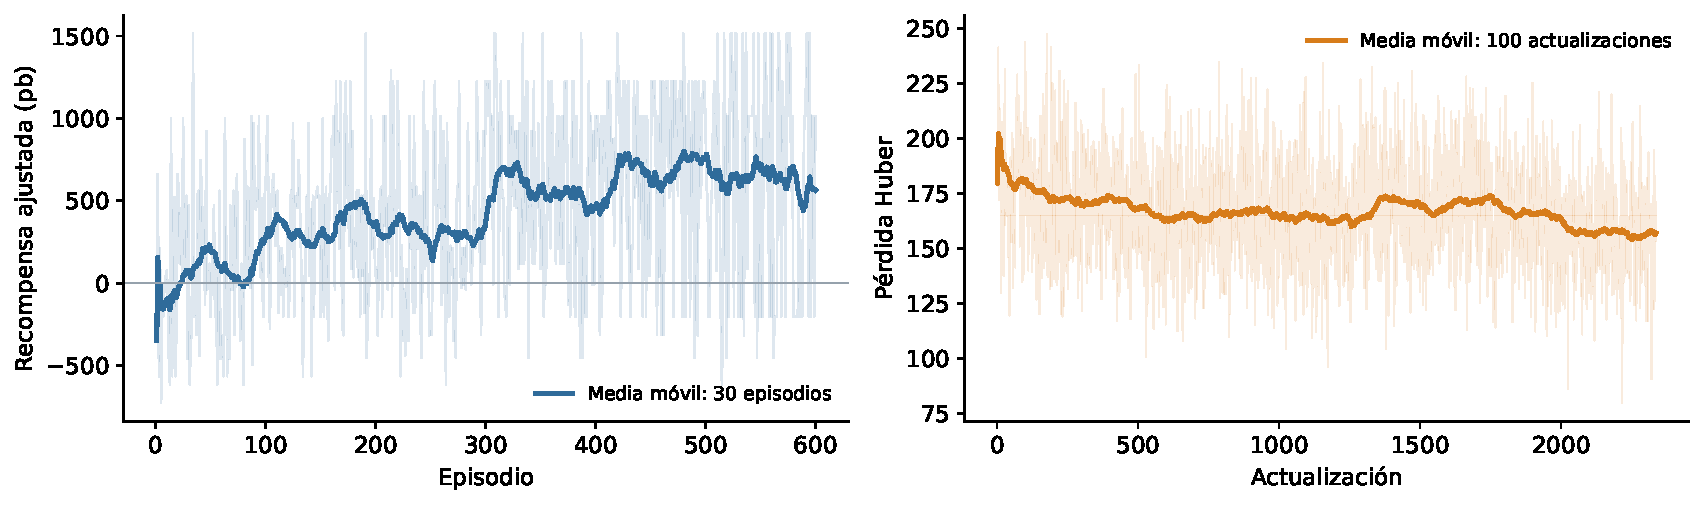
\includegraphics[width=.98\textwidth,height=.55\textheight,keepaspectratio]{dqn_entrenamiento}
\begin{itemize}\small
\item \DQNExperiencias{} experiencias; \DQNActualizaciones{} actualizaciones; \DQNSincronizaciones{} sincronizaciones.
\item La recompensa mostrada incluye el ajuste por wallets; Huber mide error frente al target.
\item Ambas curvas describen entrenamiento, no demuestran rentabilidad futura.
\end{itemize}
\end{frame}

\begin{frame}{Auditoría: una transición del replay buffer}
\begin{columns}[T,onlytextwidth]
\column{.49\textwidth}
\begin{block}{Datos de la experiencia}
\small
\begin{tabular}{lr}
\toprule
Componente & Valor \\
\midrule
Acción ejecutada & \DQNAccion \\
Recompensa inmediata & \DQNRecompensa{} pb \\
Fin del episodio & No \\
$Q_\theta(x_t,a_t)$ & \DQNPredict{} pb \\
Máximo Q futuro admisible & \DQNMaxFuturo{} pb \\
\bottomrule
\end{tabular}
\end{block}
\column{.48\textwidth}
\begin{block}{Cálculo}
\small
\[
y=\DQNRecompensa+0.99(\DQNMaxFuturo)
\]
\[
\boxed{y=\DQNTarget\ \text{pb}}
\]
\centering Pérdida de Huber: \DQNHube.
\end{block}
\end{columns}
\vspace{.5em}
\small Valores calculados con los pesos al finalizar el entrenamiento; la transición fue guardada en train.
\end{frame}


\begin{frame}{¿Qué acciones tomó el DQN en train y test?}
\centering
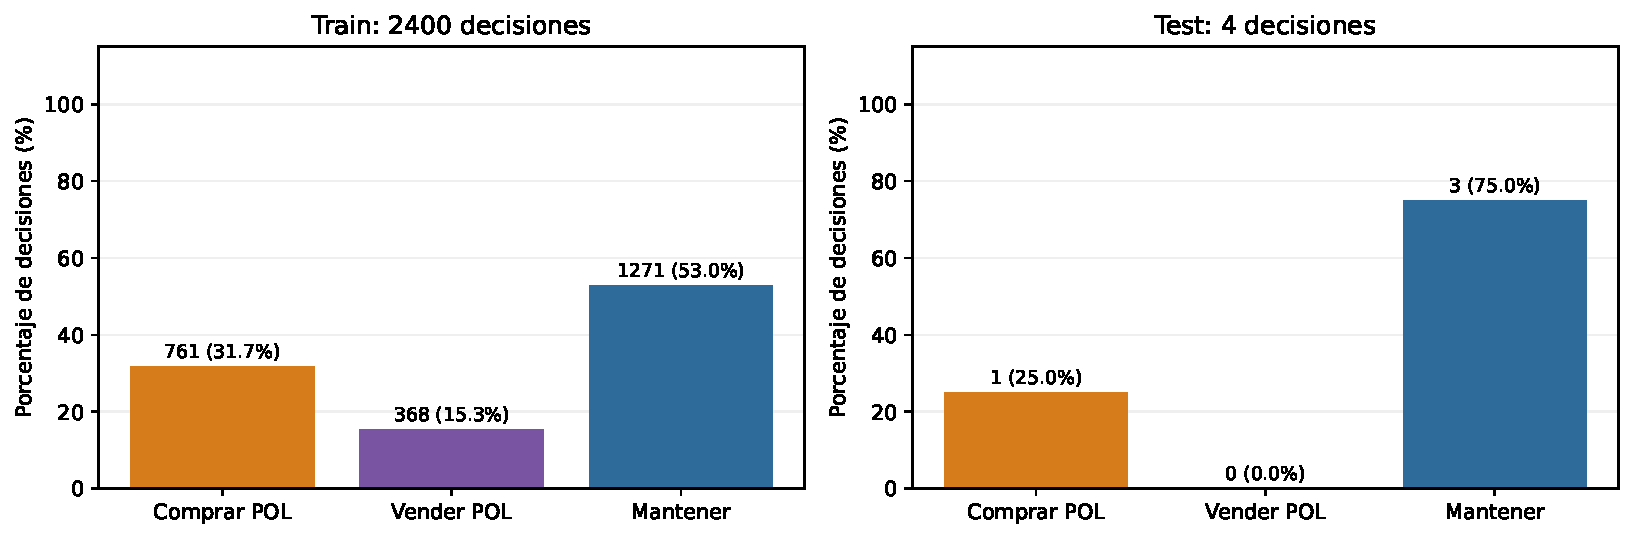
\includegraphics[width=.94\textwidth,height=.52\textheight,keepaspectratio]{dqn_acciones_train_test}
\begin{itemize}\small
\item Train: \DQNTrainDecisiones{} decisiones de episodios repetidos; \DQNTrainExploracion\% elegidas por exploración.
\item Test: \DQNTestDecisiones{} decisiones con la red congelada y sin exploración; muestra muy corta.
\item En USDC solo puede comprar o mantener; en POL, vender o mantener.
\end{itemize}
\end{frame}

\begin{frame}{¿Cómo cambian los estados?}
\centering
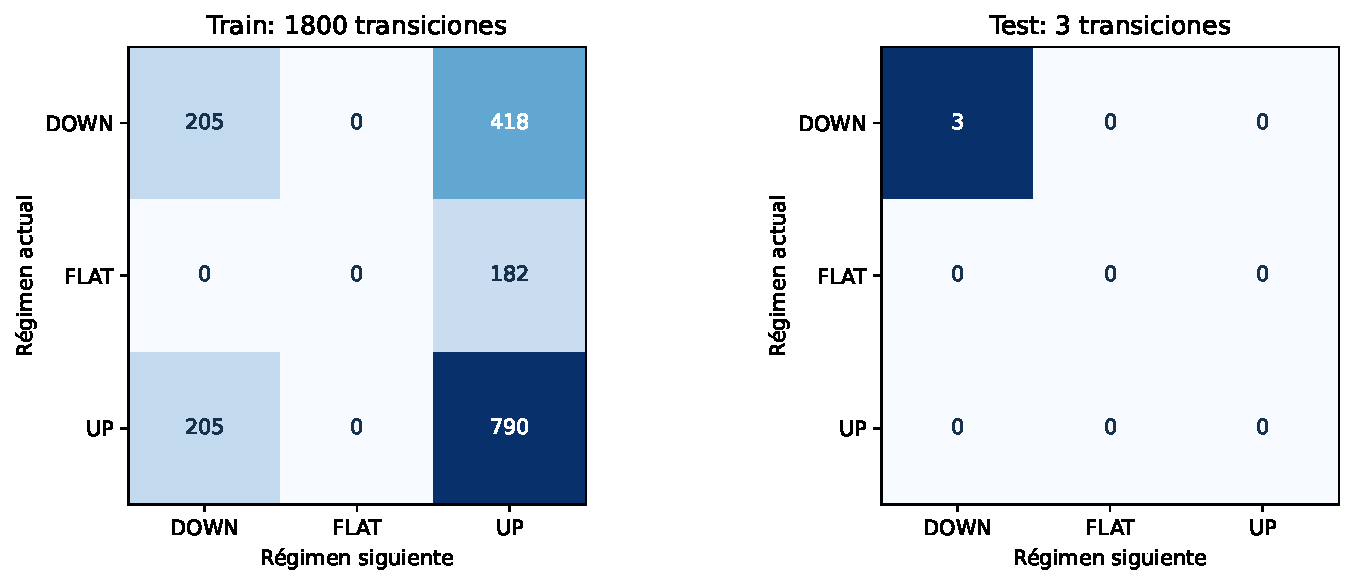
\includegraphics[width=.88\textwidth,height=.49\textheight,keepaspectratio]{dqn_transiciones_train_test}
\begin{itemize}\small
\item Filas: régimen actual; columnas: siguiente. Train: \DQNTrainTransiciones{} transiciones; test: \DQNTestTransiciones{}.
\item El estado completo incluye régimen, wallets, posición y etapa; el gráfico resume solo el régimen.
\item Test: \DQNPrimerEstado{} $\xrightarrow{\text{\DQNPrimerAccion}}$ \DQNPrimerSiguiente. El último paso es terminal.
\item Las escalas de color son independientes; el mercado siguiente no lo controla el agente.
\end{itemize}
\end{frame}

\begin{frame}{Replay histórico común: cuatro políticas sobre POL}
\centering
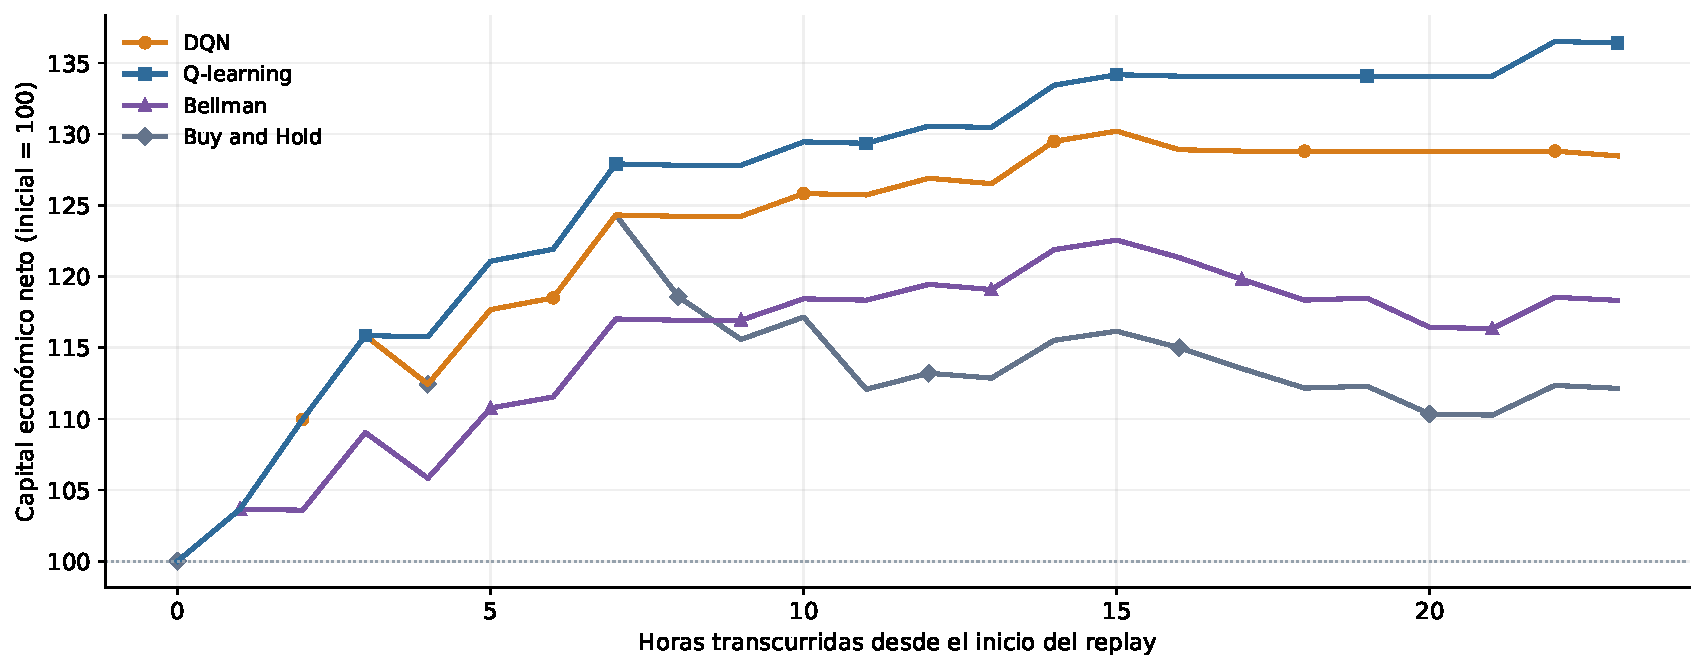
\includegraphics[width=.98\textwidth,height=.59\textheight,keepaspectratio]{replay_comun_pol}
\begin{itemize}\small
\item \DQNReplayHoras{} horas completas: \DQNReplayInicio{} a \DQNReplayFin{} UTC; capital inicial 100.
\item Los cuatro recorridos usan el mismo precio y contabilidad; la posición se mantiene entre horas.
\item Modelos entrenados en este período: replay \textbf{dentro de muestra}. Test reservado: ver anexo.
\item La última hora incompleta se excluye; curvas con el mismo capital se superponen.
\end{itemize}
\end{frame}

\begin{frame}{Sensibilidad: retirar la señal de wallets}
\centering
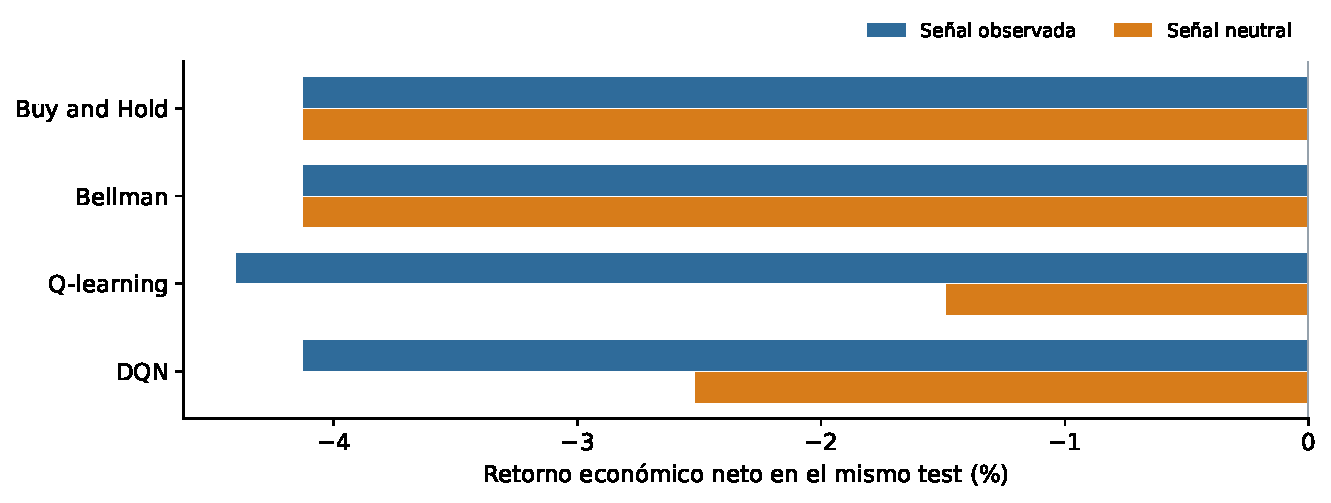
\includegraphics[width=.88\textwidth,height=.55\textheight,keepaspectratio]{dqn_estres}
\begin{itemize}\small
\item En el mismo test sustituimos la señal y los apoyos por neutral, sin reentrenar.
\item El resultado muestra sensibilidad a una intervención; no es otro test independiente.
\item Cambio DQN: $\varepsilon_{\mathrm{final}}=0.05$ y $0.30$ obtuvieron \DQNValidacionA\% y \DQNValidacionB\% en validación; se eligió \DQNEpsilon{} por desempate.
\end{itemize}
\end{frame}

\begin{frame}{Limitaciones y pasos siguientes}
\begin{columns}[T,onlytextwidth]
\column{.48\textwidth}
\begin{block}{Datos y evaluación}
\small Un solo snapshot cercano a 24 horas. Train, validación y test usan bloques de 4 horas; el test es demasiado corto para inferir desempeño futuro. Faltan auditoría temporal del ledger, slippage y profundidad.
\end{block}
\column{.48\textwidth}
\begin{block}{Modelos}
\small Bellman depende de transiciones escasas; Q tabular tiene estados sin visitas; DQN puede sobreajustar y generalizar mal. La pérdida Huber no equivale a rentabilidad.
\end{block}
\end{columns}
\vspace{.5em}
\begin{alertblock}{Siguiente comprobación}
\small Ampliar snapshots, construir períodos independientes de 24 horas y repetir validación temporal sin ajustar al test.
\end{alertblock}
\end{frame}


\begin{frame}
\centering
\vfill
{\usebeamerfont{title}\color{navy}\Large Conclusión}\par\bigskip
\begin{columns}[c,onlytextwidth]
\column{.31\textwidth}\centering\colorbox{lightpanel}{\parbox[c][1.7cm][c]{.9\linewidth}{\centering\textbf{Datos}\\[.25em]\small Swaps públicos de Polygon se convierten en perfiles.}}
\column{.34\textwidth}\centering\colorbox{lightpanel}{\parbox[c][1.7cm][c]{.9\linewidth}{\centering\textbf{Estado}\\[.25em]\small Mercado, wallets y posición dan contexto a la decisión.}}
\column{.31\textwidth}\centering\colorbox{lightpanel}{\parbox[c][1.7cm][c]{.9\linewidth}{\centering\textbf{Aprendizaje}\\[.25em]\small Q-learning actualiza valores desde experiencias horarias.}}
\end{columns}\par\bigskip
\large Bellman usa un modelo; Q-learning una tabla; DQN aproxima valores con una red.\\
Los tres requieren evaluación temporal independiente y más datos.\par\bigskip
\normalsize Gracias. Preguntas.
\vfill
\end{frame}

\appendix

\begin{frame}{Anexo: evaluación con datos reservados}
\begin{itemize}\small
\item Cuatro horas reservadas: \DQNTestInicio{} a \DQNTestFin{} UTC. Las políticas evaluadas permanecen congeladas.
\item Los modelos se entrenaron por separado de los usados en el replay histórico completo.
\end{itemize}
\vspace{.5em}
\centering
\begin{tabular}{lrr}
\hline
Método & Retorno neto & Máx. drawdown \\
\hline
DQN & \DQNTestRetDQN\% & \DQNTestDrawDQN\% \\
Q-learning & \DQNTestRetQ\% & \DQNTestDrawQ\% \\
Bellman & \DQNTestRetBellman\% & \DQNTestDrawBellman\% \\
Buy and Hold & \DQNTestRetHold\% & \DQNTestDrawHold\% \\
\hline
\end{tabular}
\vspace{1em}

\small Una prueba de cuatro horas es demasiado corta para concluir que estos resultados se repetirán.
\end{frame}

\begin{frame}{Anexo: ¿cómo se calcula el score de consistencia?}
\begin{block}{Combinación de tres componentes}
\[
\text{score}=0.50\,(\text{tasa de acierto})
+0.30\,\frac{\min(\max(PF,0),3)}{3}
+0.20\,\min\left(\frac{n}{10},1\right)
\]
\end{block}
\begin{itemize}\small
  \item \textbf{Tasa de acierto:} proporción de decisiones maduras con retorno neto positivo.
  \item \textbf{Profit factor} ($PF$): ganancias netas positivas divididas por pérdidas netas en valor absoluto; se limita a 3 para calcular el score.
  \item \textbf{Evidencia} ($n$): número de decisiones maduras; la contribución alcanza su máximo con 10.
\end{itemize}
\begin{exampleblock}{Ejemplo ilustrativo}
\small Con acierto $0.80$, $PF=1.5$ y $n=5$: score $=0.40+0.15+0.10=0.65$.
Supera el umbral general de $0.60$, pero no el $0.80$ requerido para la señal del agente.
\end{exampleblock}
\end{frame}

\begin{frame}{Anexo: nueve estados visitados en 2\,000 episodios}
\centering
\small
\renewcommand{\arraystretch}{1.13}
\begin{tabular}{lllr}
\toprule
Régimen & Señal de wallets & Posición & Visitas acumuladas \\
\midrule
DOWN & BUY & USDC & 1\,546 \\
DOWN & BUY & POL & 454 \\
DOWN & HOLD & USDC & 6\,504 \\
DOWN & HOLD & POL & 3\,496 \\
FLAT & NEUTRAL & USDC & 2\,000 \\
UP & BUY & USDC & 1\,010 \\
UP & BUY & POL & 2\,990 \\
UP & HOLD & USDC & 3\,330 \\
UP & HOLD & POL & 10\,670 \\
\midrule
\multicolumn{3}{r}{\textbf{Total}} & \textbf{32\,000} \\
\bottomrule
\end{tabular}
\renewcommand{\arraystretch}{1.0}

\vspace{.65em}
\begin{itemize}\small
  \item Cada fila agrega las visitas de una combinación $(R,W,X)$ en todas las horas y episodios.
  \item Al conservar la hora como parte de $Q_t(s,a)$, estos nueve estados forman 31 pares temporales $(t,s)$.
  \item $(\text{UP},\text{HOLD},\text{POL})$ concentró 10\,670 visitas, equivalentes al 33.34\% del entrenamiento.
\end{itemize}
\end{frame}

\begin{frame}{Anexo: registro horario del replay (1/2)}
\centering
\scriptsize
\renewcommand{\arraystretch}{1.18}
\TablaReplayPrimera\par\vspace{.55em}
\footnotesize \texttt{R/W/X} = régimen de mercado / señal de wallets / posición antes de actuar. Base, Bono y Final son retornos porcentuales por hora.
\end{frame}

\begin{frame}{Anexo: registro horario del replay (2/2)}
\centering
\scriptsize
\renewcommand{\arraystretch}{1.18}
\TablaReplaySegunda\par\vspace{.55em}
\footnotesize $X_{t+1}$ = posición después de la acción: 0=USDC y 1=POL. La columna Riqueza parte de 100 USDC y se actualiza con la recompensa final.
\end{frame}

\begin{frame}{Anexo: matriz económica de transición (1/2)}
\centering
\scriptsize
\renewcommand{\arraystretch}{1.16}
\TablaMatrizTransicionesUno\par\vspace{.45em}
\footnotesize Filas: estado económico de origen. Columnas: estado económico siguiente. Esta es la primera mitad de $P((R_{t+1},W_{t+1})\mid(R_t,W_t))$.
\end{frame}

\begin{frame}{Anexo: matriz económica de transición (2/2)}
\centering
\scriptsize
\renewcommand{\arraystretch}{1.16}
\TablaMatrizTransicionesDos\par\vspace{.45em}
\footnotesize D/F/U = DOWN/FLAT/UP; B/S/H/N = BUY/SELL/HOLD/NEUTRAL. Cada fila completa, contando ambas láminas, suma 1.
\end{frame}

\end{document}
